\documentclass{article}
\usepackage[utf8]{inputenc}
\usepackage[T1]{fontenc}
\usepackage[english]{babel}

\usepackage{amsfonts} % mathbb
\newcommand{\nn}{\mathbb{N}_n}

\newcommand{\file}[1]{\texttt{#1}}
\newcommand{\code}[1]{\texttt{#1}}
\newcommand{\clpfd}{\acrshort{clpfd}}
\newcommand{\prolog}{Prolog}
\newcommand{\sicstusprolog}{SICStus \prolog{}}
\newcommand{\srp}{\acrshort{srp}}

% Required by glossaries
% http://tex.stackexchange.com/a/93770
\usepackage{datatool}

% http://en.wikibooks.org/wiki/LaTeX/Importing_Graphics
\usepackage{graphicx}
\graphicspath{ {./graphics/} }

\usepackage{hyperref}

\usepackage{glossaries}
\newacronym{srp}{SRP}{stable roommates problem}
\newacronym{clpfd}{\code{clpfd}}{Constraint Logic Programming over Finite Domains}
\newacronym{ff}{\code{ff}}{first-fail}
\makeglossaries

\begin{document}
\title{\Acrlong{srp} solver}
\author{Filip Bártek}
\maketitle

\section{Problem definition}

Let's have $n$ participants.
Each participant knows some of the participants,
let's call these her potential partners.
Each participant has a linear ordering of her potential partners according
to preference.

Note that a participant may or may not consider herself a potential partner,
i.e. the relation of potential partnership needn't be irreflexive.

A matching is an equivalence relation on participants that has classes of size
at most 2,
i.e. assigns each participant one or none partner.
Matching must assign a potential partner to each of the participants.

An instability in a matching is a pair of participants each of whom prefers (according to their personal preference relations) the other to their current partner.

A stable matching is a matching that doesn't admit an instability.

In \acrfull{srp}, given preferences of each participant,
the task is to find a stable matching.

\subsection{Perfect matching}
A perfect matching is a matching in which every participant is assigned somebody else.

Once we can solve general \srp{},
we can force a perfect matching by making sure that no participant considers herself
a potential partner.

\section{Constraint model}
In this section we'll describe a model for \srp{} instance on $n$ participants.

We'll use the symbol $\nn$ to denote the set $\{1, \ldots, n\}$.
Each participant is uniquely identified by a number from $\nn$.

Note that the choice of variables and constraints corresponds to the capabilities
of \clpfd{}, a library that is used prominently in the implementation
of the solver.

\subsection{Variables}
\paragraph{Problem instance}
We'll represent an instance of \srp{} with $n$ participants as
a collection of preference lists $P = (P_1, \ldots, P_n)$.
$P_i$ is a preference list expressing preferences of participant $i$.
It's a $k_i$-tuple of participant identifiers (i.e. numbers from $\nn$).
All potential partners of participant $i$ are listed in $P_i$ in order of decreasing
desirability without duplicities.

\paragraph{Problem solution}
$m: \nn \rightarrow \nn$ assigns each participant her partner.

\paragraph{Auxiliary variables}
Let $s: \nn \times \nn \rightarrow \nn$ be a score function.
$s(i,j)$ represents how desirable participant $j$ is according to participant $i$.
The lower the score, the more desirable participant $j$ is.

$s$ is defined uniquely for a given instance $P$.
For every participant $i$:

\begin{itemize}
\item $j$-th potential partner is assigned score $j$
\item every participant which is not a potential partner is assigned a score $n$
\end{itemize}

As a convenience, let $\bar{s}(i)$ denote the score that participant $i$ assigns to her partner.

\subsection{Constraints}
Since the score function $s$ depends uniquely and trivially
to the problem instance $P$,
construction of $s$ from $P$ is realized
using standard \prolog{} code (without the use of \clpfd{}) and as such,
I'll leave out formal definition of the corresponding constraint.

Similarly, the properties of $P$ are not enforced formally so I'll leave out their
formal definitions.
Informal description of these properties are available in the previous section.

The following constraints constrain the solution $m$ based on $P$ and $s$:

\begin{tabular}{l | l}
Constraint & Explanation \\
\hline
$\forall i. m(i) \in P_i$ & Matching satisfies potential partners \\
$\forall i,j. m(i) = j \Leftrightarrow m(j) = i$ & Matching is symmetric \\
$\forall i. \bar{s}(i) = s(i, m(i))$ & $\bar{s}$ corresponds to $s$ and $m$ \\
$\forall i,j. \bar{s}(i) \leq s(i,j) \vee \bar{s}(j) \leq s(j,i)$ & All pairs are stable
\end{tabular}

Note especially the last of these constraints
as it captures the essence of the problem, that is the requirement of stability.
An instability occurs when a pair of participants prefer each other to their partners.
The constraint ensures that in each pair of participants,
at least one of them prefers her partner (i.e.~assigns her a lower score)
to the other participant.

\section{Implementation}
I've implemented the constraint model introduced in the previous section
using \sicstusprolog{} and its \clpfd{} library.
The implementation is available in the attached file \file{srp.pl}.

\subsection{Usage}
The main entry point is the predicate \code{srp/2}.
Its typical usage is \code{srp(Preferences, Matching)},
where \code{Preferences} is a fully instantiated list of ordered lists
of potential partners
and \code{Matching} is unbound.
If a solution of \srp{} instance described by \code{Preferences} exists,
it is unified with \code{Matching}.
Otherwise \code{srp} fails.

Internally, \code{srp} uses \clpfd{} library to search for the solution.
The searching procedure executed by \code{clpfd:labeling/2}
can optionally be customized by passing a list of options in the first argument
of \code{labeling}.
This argument of \code{labeling} is exposed
in the third argument of the extended \code{srp/3}.
For example, one may execute \code{srp(Preferences, Matching, [ffc, assumptions(K)])}.

\subsection{Correctness}
Correctness of the implementation was assessed using a set of tests on small
manually constructed and solved \srp{} instances (up to size 8).

The tests are bundled in the source file \file{srp.pl}
and can be accessed using \code{plunit} library interface
(typically by executing \code{plunit:run\_tests.}).

\subsection{Performance}
I've examined the performance of the solver using various problem instances
(esp.~of various sizes) and search strategies.

\subsubsection{System configuration}
The performance measurements were performed on a computer
with the following configuration:

\begin{tabular}{| l | l |}
\hline
Model & HP Compaq 6510b \\
\hline
CPU & Intel Core2 Duo T8100 2.10 GHz \\
\hline
RAM & 2.50 GB \\
\hline
Operating system & Windows Vista Business 32-bit \\
\hline
\sicstusprolog{} & 4.2.3 \\
\hline
\end{tabular}

\subsubsection{Instance generation}
For the purposes of measuring performance of the solver,
instances of \acrshort{srp} were generated randomly in the following manner:
for a given $n$, each of the $n$ participants' preference lists
is a random permutation of $\nn$
such that every possible permutation occurs with equal probability.

\subsubsection{Measurement procedure}
The following instance sizes (values of $n$) were examined:
0, 1, 2, 4, 8, 16, 24, 32, 40, 48 and 64.

For every examined value of $n$, 10 random instances were generated.
Each of these instances was solved using each of the three relevant basic
search strategies offered by \code{clpfd:labeling/2}:

\begin{itemize}
\item \code{leftmost},
\item \acrshort{ff} (\acrlong{ff}) and
\item \code{ffc} (most constrained).
\end{itemize}

Two values were measured: \emph{time to find a solution}
and \emph{number of assumptions}.

Time was measured using \sicstusprolog{} built-in predicate \code{statistics/2}
with keyword \code{runtime}.
%TODO: Verify.
The solving procedure was repeated 100 times on each instance;
the reported times are averages from these 100 executions.

Assumptions are the choices made by \code{clpfd:labeling/2} during the search for
a solution.
Their number is extracted from the search procedure using the option
\code{assumptions(K)}.

In all cases, the solver was only run until it found the first solution.
In cases the solver couldn't find any solution,
no measurements were performed for that instance.

\subsubsection{Results}

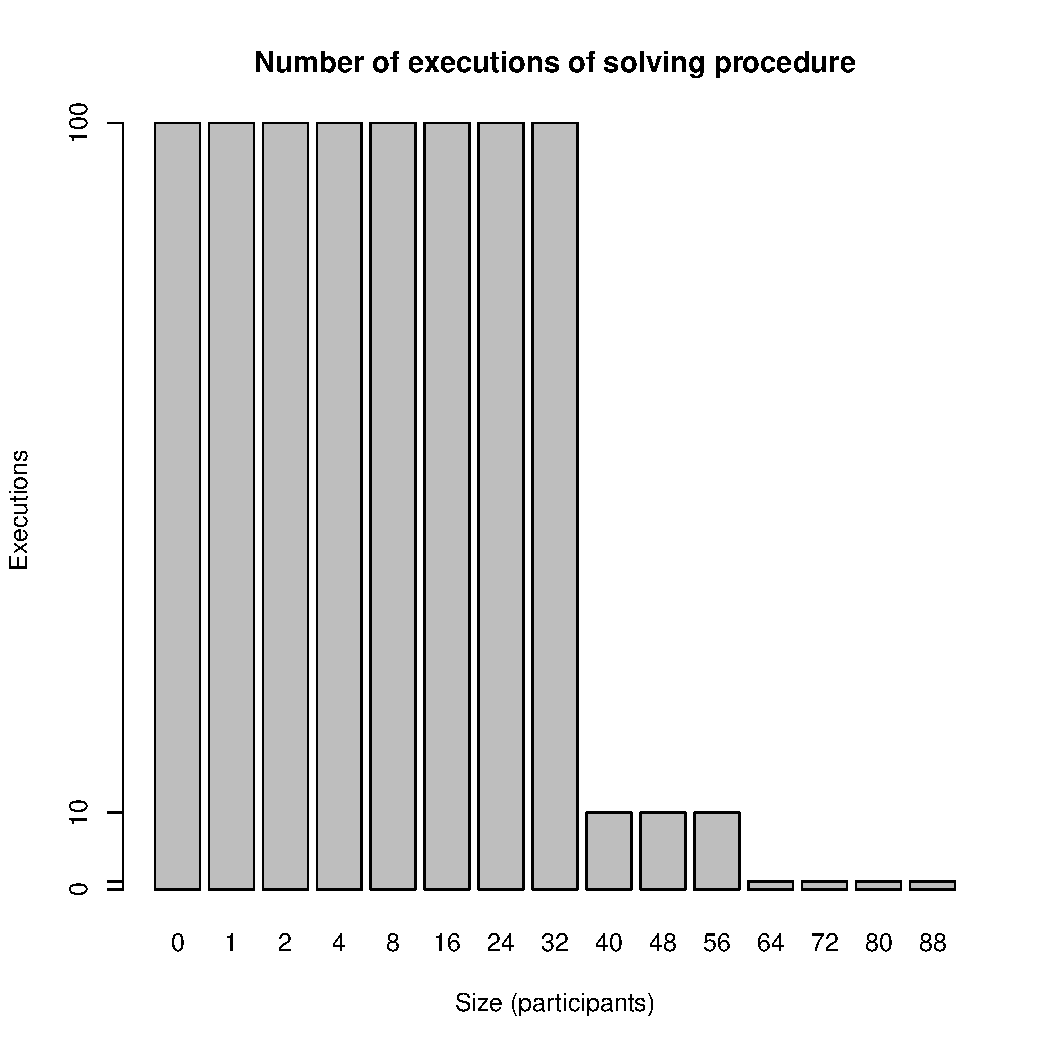
\includegraphics[width=\linewidth]{executions}

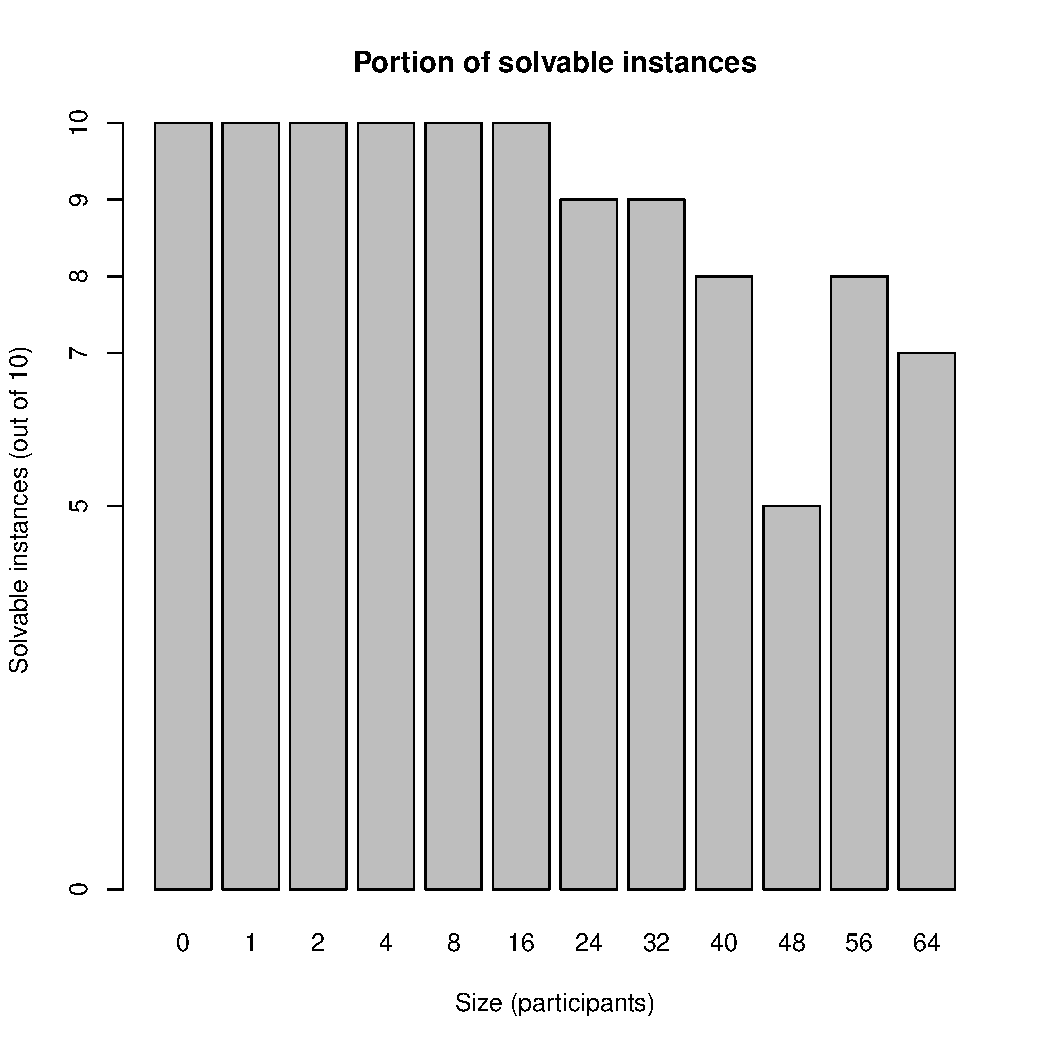
\includegraphics[width=\linewidth]{solvable}

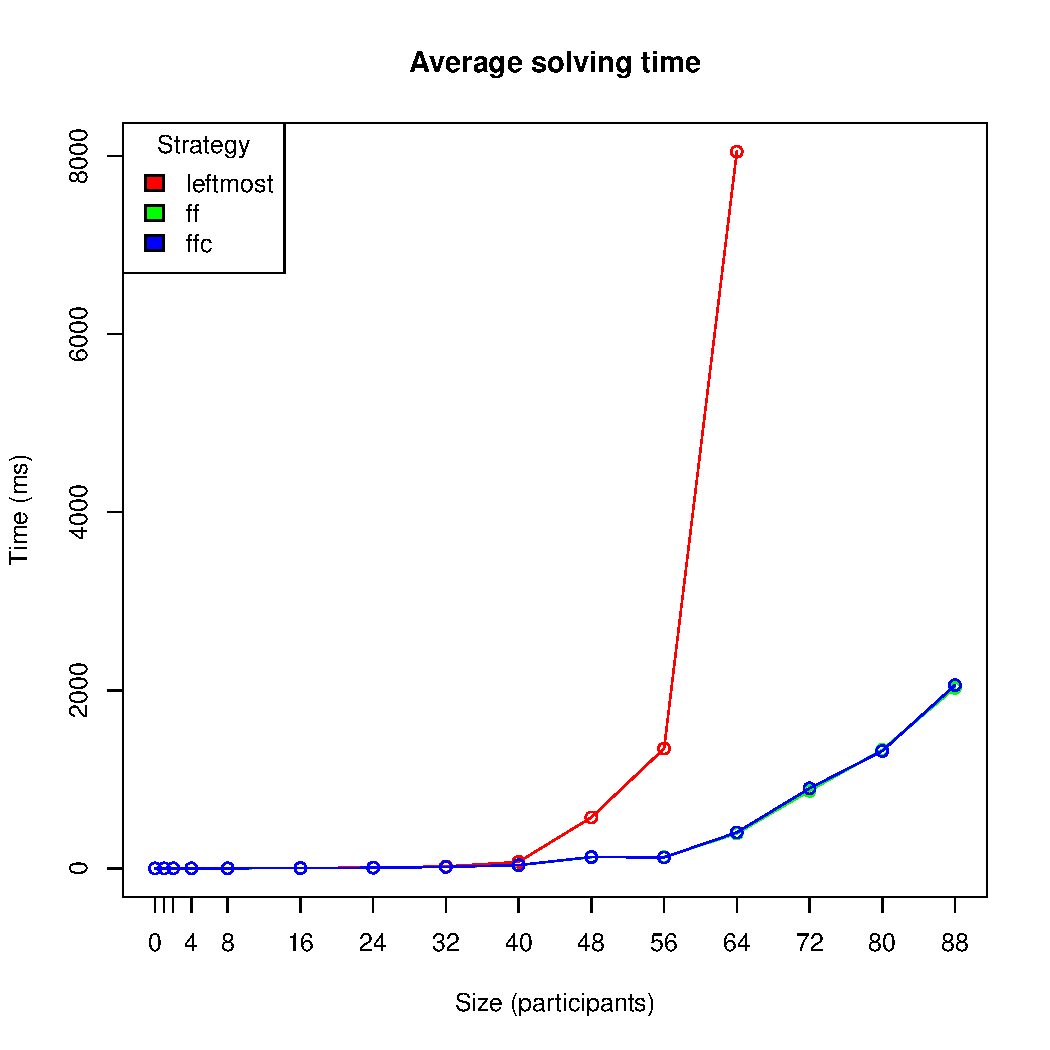
\includegraphics[width=\linewidth]{time}

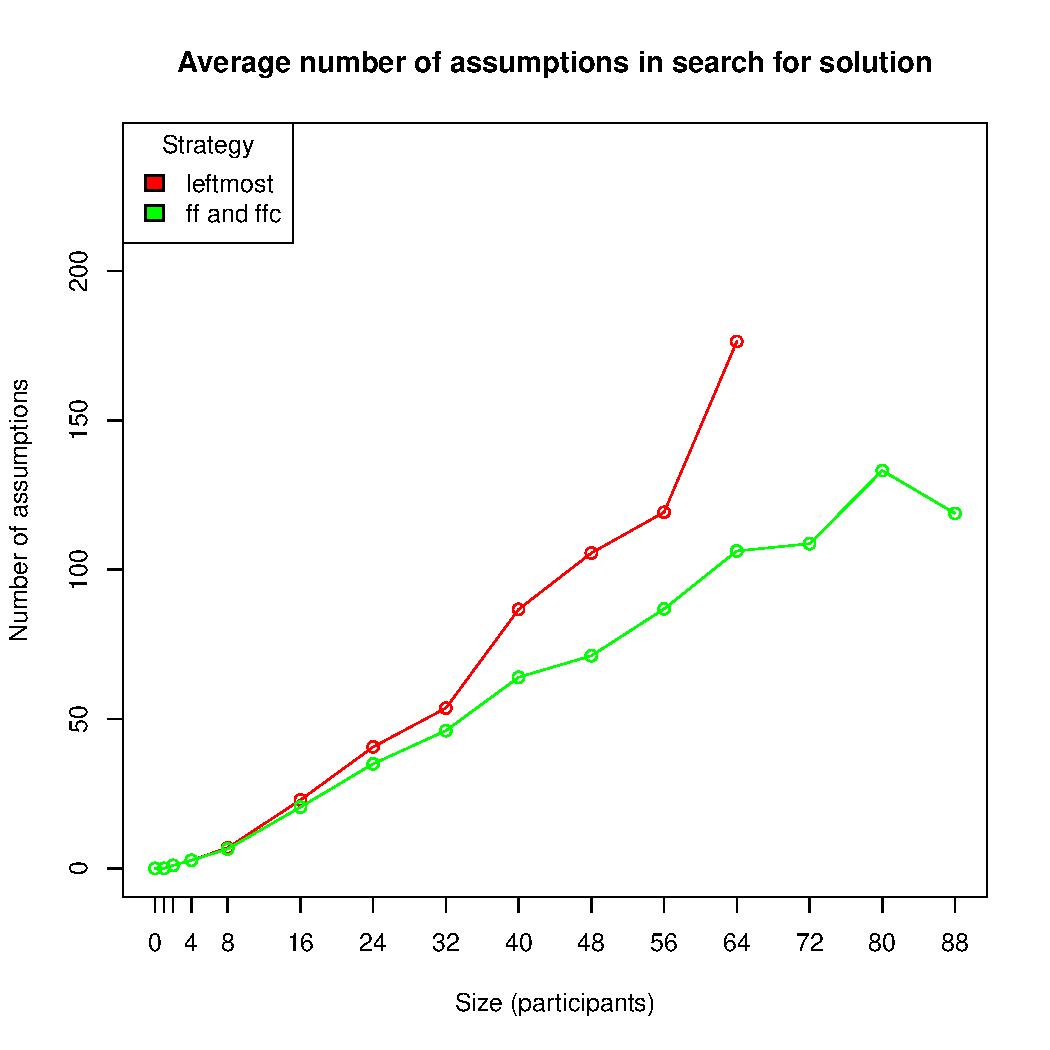
\includegraphics[width=\linewidth]{assumptions}

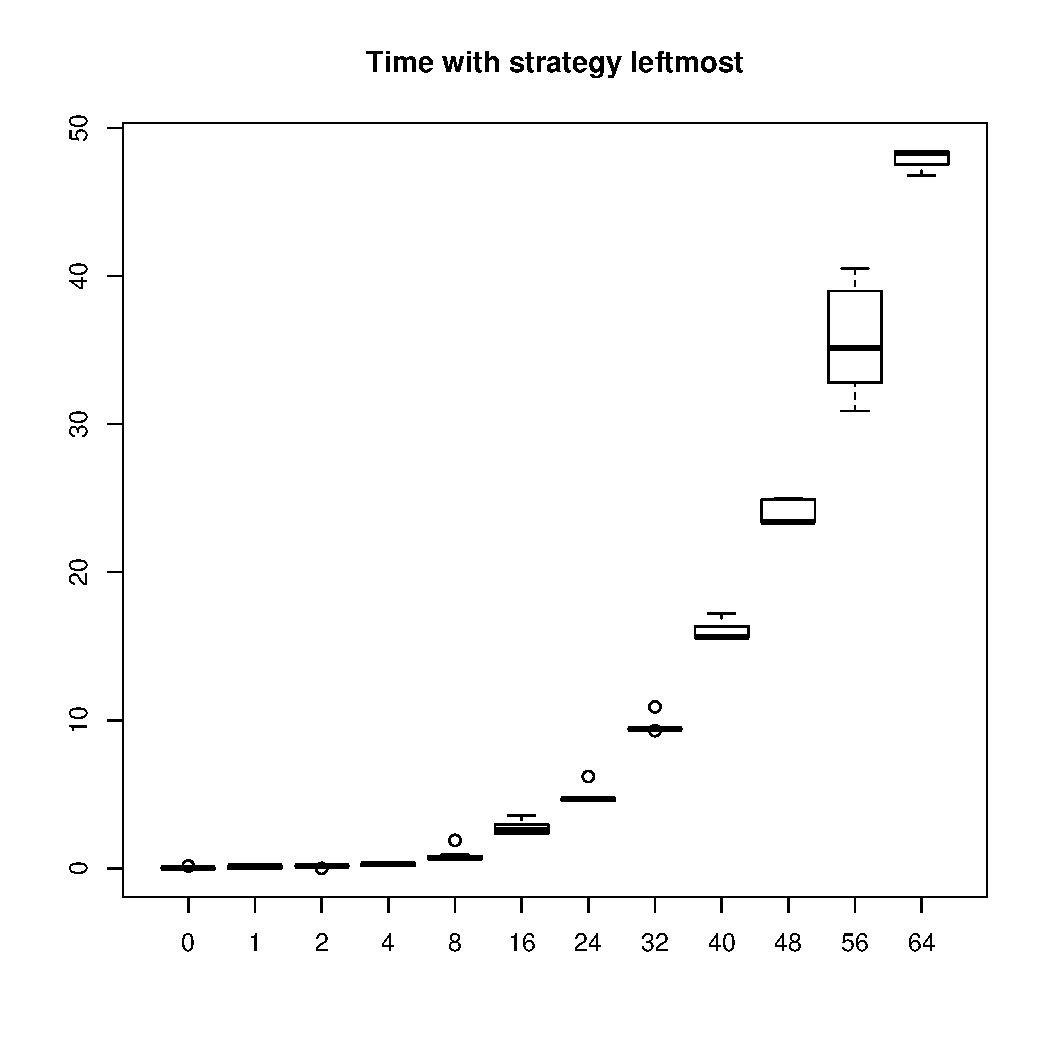
\includegraphics[width=\linewidth]{leftmost_time}

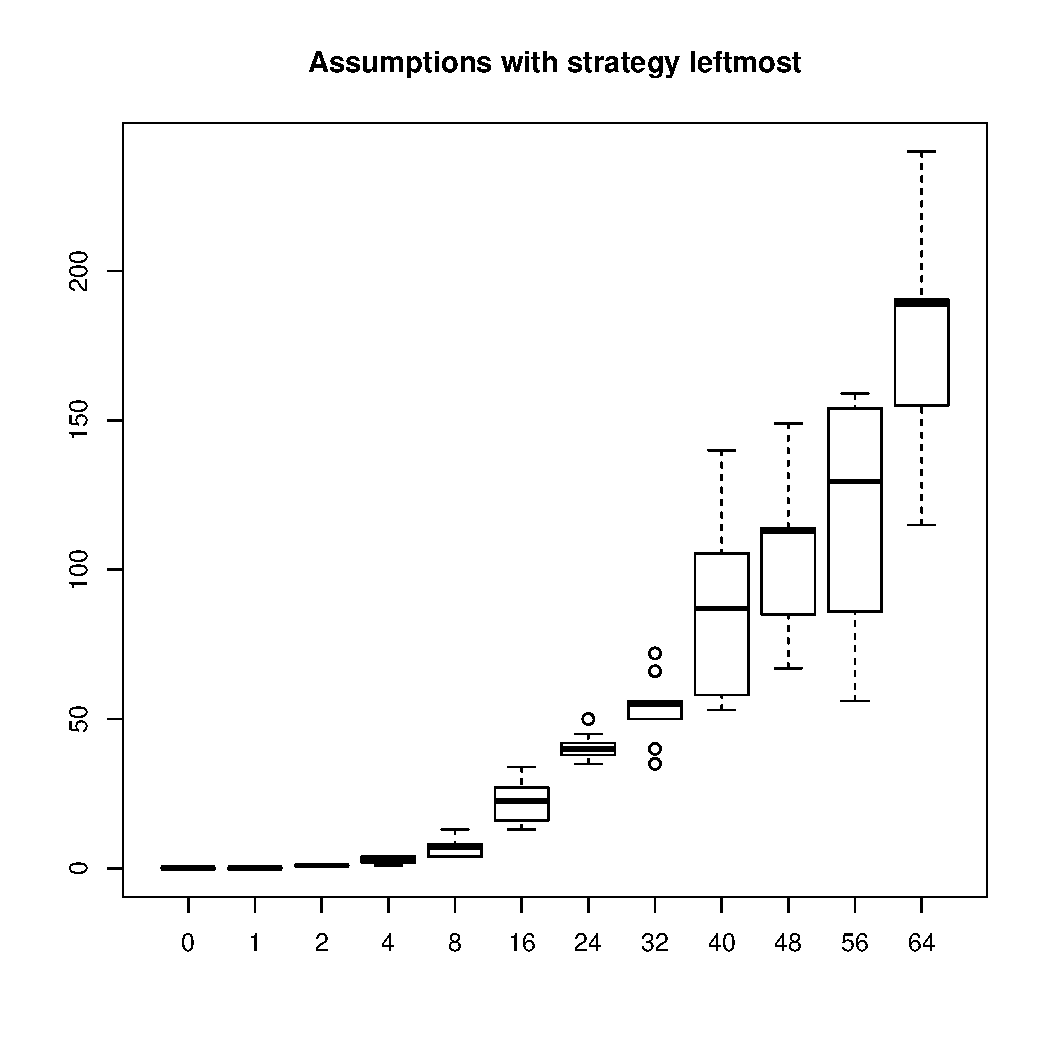
\includegraphics[width=\linewidth]{leftmost_assumptions}

%TODO: Finish.

\printglossaries{}

\end{document}
